\hypertarget{a00830}{}\section{Pro Tools Guide}
\label{a00830}\index{Pro Tools Guide@{Pro Tools Guide}}
Details about using A\+AX plug-\/ins in Pro Tools. 

\hypertarget{a00830_aax_pro_tools_guide_contents}{}\subsection{Contents}\label{a00830_aax_pro_tools_guide_contents}
\begin{DoxyItemize}
\item \mbox{\hyperlink{a00830_aax_pro_tools_guide_00_about_this_document}{About this document}} \item \mbox{\hyperlink{a00830_aax_pro_tools_guide_01_processing_modes}{Processing modes}} \item \mbox{\hyperlink{a00830_aax_pro_tools_guide_02_requirements_for_aax_plugin_compatibility_with_pro_tools}{Requirements for A\+AX plug-\/in compatibility with Pro Tools}} \item \mbox{\hyperlink{a00830_aax_pro_tools_guide_03_audio_engine_behavior}{Audio Engine Behavior and Features}} \item \mbox{\hyperlink{a00830_aax_pro_tools_guide_04_basic_plugin_operation}{Basic plug-\/in operation}} \item \mbox{\hyperlink{a00830_aax_pro_tools_guide_05_optional_plugin_features}{Optional plug-\/in features}} \item \mbox{\hyperlink{a00830_aax_pro_tools_guide_06_debugging_aax_plugins}{Debugging A\+AX plug-\/ins}} \item \mbox{\hyperlink{a00830_aax_pro_tools_guide_06b_troubleshooting_aax_plugin_failures}{Troubleshooting common A\+AX plug-\/in failures}} \item \mbox{\hyperlink{a00830_aax_pro_tools_guide_06c_digioptions}{Using Digi\+Options}} \item \mbox{\hyperlink{a00830_aax_pro_tools_guide_07_compatibility_notes}{Compatibility Notes}}\end{DoxyItemize}
 \hypertarget{a00830_aax_pro_tools_guide_00_about_this_document}{}\subsection{About this document}\label{a00830_aax_pro_tools_guide_00_about_this_document}
This guide discusses specific details related to using A\+AX plug-\/ins with Pro Tools, such as loading and initialization procedures, G\+UI hosting, and other application-\/specific features. This guide is not intended to provide complete documentation for the Pro Tools application. For more information about the features, functionality, and use of Pro Tools see the Pro Tools Reference Guide, available for download from the Avid web site.

{\itshape This guide is a work in progress, and is extended as needed to describe different aspects of and caveats to the Pro Tools implementation of the A\+AX host spec.} 

 \hypertarget{a00830_aax_pro_tools_guide_01_processing_modes}{}\subsection{Processing modes}\label{a00830_aax_pro_tools_guide_01_processing_modes}
Pro Tools supports three A\+AX processing modes\+: Audio\+Suite, A\+AX Native, and A\+AX D\+SP. 
\begin{DoxyItemize}
\item Audio\+Suite plug-\/ins perform non-\/real-\/time, random-\/access, file-\/based processing entirely on the host C\+PU.  
\item A\+AX Native plug-\/ins perform real-\/time, linear, non-\/destructive processing entirely on the host C\+PU. Native plug-\/ins are also used by Pro Tools to perform offline rendering.  
\item D\+SP plug-\/ins perform real-\/time, linear, non-\/destructive processing on D\+S\+P-\/accelerated hardware, with non-\/real-\/time tasks performed on the host C\+PU.  
\end{DoxyItemize}

Each of these processing modes offers specific advantages and trade-\/offs in functionality, power, and development effort, and plug-\/in developers may choose to develop only for specific processing modes if the features provided by those modes are required by the plug-\/in.

\hypertarget{a00830_subsection__realtime_processing}{}\subsubsection{Real-\/time processing}\label{a00830_subsection__realtime_processing}
 Real-\/time processing allows users to operate plug-\/ins in live signal paths or in complicated audio routing schemes when the future input data is not known.

Plug-\/ins operating in real-\/time are clients of the Pro Tools automation system, meaning that control movements can be dynamically recorded and played back with the audio track, written by hand onto the Pro Tools timeline for future playback, and/or edited by and broadcast to attached control surfaces.

To instantiate a plug-\/in for real-\/time processing in Pro Tools, click on an insert slot in the desired track and select the plug-\/in from the menu that appears

\hypertarget{a00830_subsubsection__native_realtime_processing_}{}\paragraph{Native real-\/time processing}\label{a00830_subsubsection__native_realtime_processing_}
 When an A\+AX plug-\/in is run natively, all of its components and processing elements are loaded into the host environment. The host C\+PU handles the plug-\/in\textquotesingle{}s real-\/time audio processing as well as its data model, G\+UI, and other tasks.

\hypertarget{a00830_subsubsection__dsp_realtime_processing_}{}\paragraph{D\+S\+P real-\/time processing}\label{a00830_subsubsection__dsp_realtime_processing_}
 When an A\+AX plug-\/in is run with Avid\textquotesingle{}s D\+S\+P-\/enabled hardware, the plug-\/in\textquotesingle{}s real-\/time processing code is loaded onto the external D\+SP device, while the remaining plug-\/in modules continue to be run by the host C\+PU. Each D\+SP in this system provides dedicated processing capacity that is not shared with an OS or other processes, and therefore this architecture allows users to achieve highly reliable and deterministic low-\/latency processing even when many D\+SP plug-\/ins are instantiated.

~

~   Figure 1\+: Real-\/time insert slots in the Pro Tools Edit and Mix windows.

\hypertarget{a00830_subsubsection__cpu_reporting_}{}\paragraph{C\+P\+U reporting}\label{a00830_subsubsection__cpu_reporting_}
 To guarantee absolute reliability, A\+AX D\+SP plug-\/ins are required to report their worst-\/case performance metrics to Pro Tools. Pro Tools uses this information to ensure that each D\+SP in the system will be loaded with only the number of plug-\/ins that it can support given a worst-\/case processing load.

\hypertarget{a00830_subsection__non-real-time_processing_audiosuite}{}\subsubsection{Non-\/real-\/time processing (\+Audio\+Suite)}\label{a00830_subsection__non-real-time_processing_audiosuite}
 The non-\/real-\/time Audio\+Suite processing mode is file-\/based, meaning that the results of Audio\+Suite processing are applied destructively to audio files (generally to new, empty files provided by Pro Tools.) Audio\+Suite processing can only be performed on preexisting blocks of audio.

There are two primary ways to apply Audio\+Suite processing in Pro Tools. The first way is to selectively apply the processing algorithm to the audio tracks and clips that are selected on the Pro Tools timeline. This is known as \char`\"{}destructive\char`\"{} processing, because the original audio track is replaced by the new processed audio track. There are no limitations governing the amount of time required to process a track in this manner.

Audio Suite plug-\/ins also have a second optional mode in which they can run. This is referred to as Preview mode. The Preview feature allows you to monitor the audio processing applied to a track in semi-\/real-\/time. Because this is a real-\/time process, it is not applicable to all types of file based processing. You may elect not to support this mode in your plug-\/in if its algorithm does not lend itself to real-\/time, linear processing. Preview mode is implemented in a non-\/ destructive manner, as Preview mode exists for auditioning only with no actual replacement of audio data on the Pro Tools timeline.

To instantiate an Audio\+Suite plug-\/in in Pro Tools, select the plug-\/in from the \char`\"{}\+Audio\+Suite\char`\"{} menu in the Pro Tools application menu bar

\hypertarget{a00830_subsection__multichannel_and_multimono}{}\subsubsection{Multichannel and Multi-\/\+Mono}\label{a00830_subsection__multichannel_and_multimono}
 Pro Tools supports various surround stem formats throughout the entire signal chain, including multi-\/channel processing through A\+AX plug-\/ins.

Pro Tools also allows a plug-\/in to function in multi-\/mono mode if the plug-\/in does not explicitly support certain channel formats. In multi-\/mono mode, Pro Tools instantiates a separate instance of a plug-\/in for every channel in the track. In this mode, plug-\/in controls across all channel-\/instances in a multi-\/mono collection are linked by default, though channels can be unlinked by toggling the blue link button in the plug-\/in header and selecting the channel whose controls you wish to modify.

For more information about multi-\/mono mode, please refer to the Pro Tools Reference Guide.



 \hypertarget{a00830_aax_pro_tools_guide_02_requirements_for_aax_plugin_compatibility_with_pro_tools}{}\subsection{Requirements for A\+A\+X plug-\/in compatibility with Pro Tools}\label{a00830_aax_pro_tools_guide_02_requirements_for_aax_plugin_compatibility_with_pro_tools}
 In addition to implementing the client-\/side A\+AX A\+PI, all Pro Tools plug-\/ins must\+: 
\begin{DoxyEnumerate}
\item Be installed to the A\+AX plug-\/ins directory  
\item Use a valid file name 
\item Be signed with a valid digital signature \begin{DoxyNote}{Note}
Digital signatures for plug-\/ins are not required in Pro Tools developer builds  
\end{DoxyNote}

\end{DoxyEnumerate}

\hypertarget{a00830_subsection__install_directories_}{}\subsubsection{Install directories}\label{a00830_subsection__install_directories_}
 A\+AX plug-\/ins must be installed in the system\textquotesingle{}s A\+AX Plug-\/\+Ins directory. See \mbox{\hyperlink{a00843_aax_distributing_installer}{Building your plug-\/in installer}} for more information about creating a plug-\/in installer.

Plug-\/ins that are uninstalled but still present on the system are placed into the \char`\"{}\+Plug-\/\+Ins (\+Unused)\char`\"{} directory, which is located next to the Plug-\/\+Ins directory.

Pro Tools will also search for a Plug-\/\+Ins directory next to the actual Pro Tools application, and this directory will be used if present. This debug feature can be useful for testing specific plug-\/ins.

\hypertarget{a00830_subsection__file_name_}{}\subsubsection{Plug-\/in name and file structure}\label{a00830_subsection__file_name_}
 In order to be recognized by A\+AE, all A\+AX plug-\/in bundles must use the \char`\"{}.\+aaxplugin\char`\"{} file name suffix. On OS X, the plug-\/in bundle must use this suffix while the binary itself does not require a suffix. On Windows, the plug-\/in binary (D\+LL) must use this suffix.

The directory structure of an A\+AX plug-\/in bundle is also important. See \mbox{\hyperlink{a00801_commoninterface_formatspecification__aaxplugin_directory_structure}{.aaxplugin Directory Structure}} in the \mbox{\hyperlink{a00801}{A\+AX Format Specification}} document for more information.

\hypertarget{a00830_subsection__digital_signature_}{}\subsubsection{Digital signature}\label{a00830_subsection__digital_signature_}
 As an added security measure against digital piracy, all A\+AX plug-\/in binaries must be digitally signed in order to run in Pro Tools. This signature step does not interfere with your existing copy protection and licensing solutions -\/ it is simply a build step that you incorporate into your plug-\/in before releasing the binary.

Digital signatures are generated based on the plug-\/in binary and act as a guarantee against binary modification. Therefore, any build steps that modify the binary, such as symbol stripping, must be performed prior to signature generation. Digital signatures apply to the full .aaxplugin bundle, so any operation that modifies the contents of the bundle will invalidate its digital signature even if the operation does not affect the plug-\/in binary itself. Therefore, the generation and application of a digital signature should be the last step in any release plug-\/in build process.

\begin{DoxyNote}{Note}
The digital signature requirement applies to Beta and Release software. This requirement does not apply to Development builds of Pro Tools or to other developer tools which can load unsigned binaries.
\end{DoxyNote}
If you are having problems with digitally signing your plug-\/ins see the \mbox{\hyperlink{a00842_troubleshooting_signature}{Plug-\/\+In Fails to Load in Shipping Pro Tools}} section in the \mbox{\hyperlink{a00842}{Troubleshooting}} guide.

 Requesting the digital signing toolkit

The A\+AX digital signatures required by Pro Tools are generated using digital signing tools licensed from P\+A\+CE Anti-\/\+Piracy, Inc., which acts as the certificate authority for all A\+AX digital signatures. To request access to these tools, send an e-\/mail to \href{mailto:partners@avid.com?subject=Pace Tools Request}{\texttt{ partners@avid.\+com}} with \char`\"{}\+Pace Tools Request\char`\"{} in the subject. Include the following information in your request\+:


\begin{DoxyItemize}
\item Company name
\item Company mailing address
\item Contact information for your A\+AX development lead or team
\item i\+Lok username which you will use for your digital signing admin account
\end{DoxyItemize}

Once your request has been approved you will be contacted by P\+A\+CE with further instructions for acquiring and using the digital signature toolkit.

 What you will need

The digital signing toolkit which you will receive as an A\+AX developer will require a physical i\+Lok U\+SB key. You will also need a registered i\+Lok user account which will be used when applying the digital signature. If your build toolchain requires hardware-\/free signing then you can contact P\+A\+CE regarding their current offerings.

In order to successfully use the signing tools you should be familiar with the latest Gatekeeper and {\ttfamily codesign} (for Mac) and Authenticode (for Windows) digital signature schemes.

Although it is possible to use self-\/signed certificates for A\+AX digital signatures, before making your A\+AX plug-\/ins commercially available it is recommended that you acquire an Apple-\/issued Application Developer ID for Gatekeeper and an \char`\"{}\+Extended Verification\char`\"{} (EV) Authenticode certificate from a Microsoft approved certificate authority.

See the Getting Started Guide in the P\+A\+CE digital signing toolkit for more information about using these tools.

 Signature requirements in Pro Tools 11

 \begin{DoxyRefDesc}{Host Compatibility Notes}
\item[\mbox{\hyperlink{a00786__compatibility_notes000012}{Host Compatibility Notes}}]Pro Tools 11 requires P\+A\+CE Eden digital signatures for A\+AX plug-\/ins.\end{DoxyRefDesc}


Pro Tools 11 and higher use the Eden toolset. This toolset integrates fully with platform-\/specific signatures, so you only need to do one post-\/build step using the Eden digital signing tools to sign your plug-\/in with both the Eden signature and the relevant Apple Gate\+Keeper or Microsoft Authenticode signature. For more information, see the Eden digital signature toolkit documentation.

Pro Tools 11 and higher will only accept the Eden signature; A\+AX plug-\/ins signed by earlier generations of P\+A\+CE digital signing tools will not load in Pro Tools 11.

 Signature requirements in Pro Tools 10

 \begin{DoxyRefDesc}{Host Compatibility Notes}
\item[\mbox{\hyperlink{a00786__compatibility_notes000013}{Host Compatibility Notes}}]Pro Tools 10 requires either P\+A\+CE D\+Sig or Eden digital signatures for A\+AX plug-\/ins.\end{DoxyRefDesc}


For compatibility with Pro Tools 10, A\+AX plug-\/ins must be digitally signed using P\+A\+C\+E\+D\+Sig\+Tool.

Pro Tools 10.\+3.\+5 and above also support the new Eden signatures from P\+A\+CE, so that universal binaries can be shipped which target both Pro Tools 11 or later and Pro Tools 10.\+3.\+5 or later.

 Optional Signature for Pro Tools A\+AX D\+SP binaries

 \begin{DoxyRefDesc}{Host Compatibility Notes}
\item[\mbox{\hyperlink{a00786__compatibility_notes000014}{Host Compatibility Notes}}]As of Pro Tools 10.\+2, support has been added to allow binary-\/level encryption of A\+AX D\+SP algorithms. Please note that this is {\itshape N\+OT} a requirement of A\+AX D\+SP plug-\/ins, and serves only as an additional security measure to protect an algorithm\textquotesingle{}s D\+LL. \end{DoxyRefDesc}


For more information about signing A\+AX plug-\/ins for use with Pro Tools 10, please contact P\+A\+CE.

 Automatic signature application by P\+A\+CE tools

If you already protect your plug-\/ins using one of the anti-\/piracy technologies available from P\+A\+CE then you may not need to perform any additional action\+:


\begin{DoxyItemize}
\item you are wrapping using P\+A\+CE Inter\+Lok Master\+Maker, your binaries will be automatically signed.  
\item If you are using Fusion Hybrid without wrapping with Master\+Maker, please carefully review the \char`\"{}\+Adding digital signature checks\char`\"{} section of the Fusion Hybrid manual.  
\item If you are using P\+A\+CE A\+P\+Is (like P\+A\+CE Interface or C\+D\+RM) without Inter\+Lok wrapping, please see either the latest P\+A\+C\+E\+D\+Sig\+Tool read me or the Fusion Hybrid manual for additional details regarding digital signing.  
\end{DoxyItemize}



 \hypertarget{a00830_aax_pro_tools_guide_03_audio_engine_behavior}{}\subsection{Audio Engine Behavior and Features}\label{a00830_aax_pro_tools_guide_03_audio_engine_behavior}
 Pro Tools hosts A\+AX plug-\/ins using the {\itshape  Avid Audio Engine} (A\+AE). A\+AE implements all host-\/side A\+AX interfaces such as \mbox{\hyperlink{a01789}{A\+A\+X\+\_\+\+I\+Controller}} and the \mbox{\hyperlink{a01777}{A\+A\+X\+\_\+\+I\+Collection}}.

\hypertarget{a00830_subsection__plugin_loading_and_aae_initialization}{}\subsubsection{Plug-\/in loading and A\+A\+E initialization}\label{a00830_subsection__plugin_loading_and_aae_initialization}
 When Pro Tools launches, it immediately begins loading A\+AE. A\+AE searches the system for valid A\+AX plug-\/ins, checks each plug-\/in\textquotesingle{}s digital signature, and loads, initializes and catalogs any valid plug-\/in modules that it happens to find.

This initialization is performed via the plug-\/in\textquotesingle{}s Describe implementation; once A\+AE loads a plug-\/in binary, it calls the plug-\/in\textquotesingle{}s Describe method to retrieve (and cache) the basic configuration of the plug-\/in. A\+AE then hands this information back to Pro Tools so that Pro Tools knows what plug-\/ins are available and what their basic properties are. Once a complete list of plug-\/in descriptions has been generated, A\+AE can construct any plug-\/in\textquotesingle{}s individual modules and manage its algorithm.

\hypertarget{a00830_subsubsection__plugin_configuration_cacheing_}{}\paragraph{Plug-\/in configuration cacheing}\label{a00830_subsubsection__plugin_configuration_cacheing_}
 A\+AE is pretty smart, and it knows during initialization if anything has changed within the A\+AE Plug-\/\+Ins folder since the last time it was run. If nothing has changed, A\+AE relies on plug-\/in descriptions that it cached during the previous launch to speed through the plug-\/in loading process. If, however, any plug-\/ins have been added, removed, or updated since the last launch, A\+AE loads and re-\/caches the description for every installed plug-\/in.

\begin{DoxyNote}{Note}
We recommend that you always enable the {\ttfamily Always\+Rebuild\+Cache} Digi\+Option during plug-\/in development. See \mbox{\hyperlink{a00830_aax_pro_tools_guide_06c_digioptions}{Using Digi\+Options}} for more information.
\end{DoxyNote}
\hypertarget{a00830_subsection__plugin_initialization}{}\subsubsection{Plug-\/in initialization}\label{a00830_subsection__plugin_initialization}
 When a new plug-\/in instance is created in Pro Tools, A\+AE performs the following steps\+: 
\begin{DoxyEnumerate}
\item The plug-\/in\textquotesingle{}s data model component is loaded  
\item The default state of the plug-\/in is set (see \mbox{\hyperlink{a00830_subsubsection__default_plugin_settings_}{Default plug-\/in settings}})  
\item The plug-\/in\textquotesingle{}s G\+UI and other host modules are loaded  
\item The plug-\/in\textquotesingle{}s algorithm private data state is initialized  
\item The plug-\/in\textquotesingle{}s algorithm is loaded and initialized  
\item The plug-\/in\textquotesingle{}s algorithm processing is initiated 
\end{DoxyEnumerate}

\hypertarget{a00830_subsection__runtime_processing_behavior}{}\subsubsection{Run-\/time processing behavior}\label{a00830_subsection__runtime_processing_behavior}
  Pro Tools 11 The audio engine in Pro Tools 11 includes some advanced real-\/time processing features that are not present in earlier versions of Pro Tools\+:


\begin{DoxyItemize}
\item When certain tracks with plug-\/ins have been silent for a period of time or Pro Tools is not in playback, those plug-\/in instances are automatically deactivated to reduce processing load on the host processor  
\item In certain situations such as playback or offline bounce where low latency is not required, Pro Tools may call A\+AX Native plug-\/ins with a larger buffer than normal. 
\end{DoxyItemize}

This latter behavior is possible due to the fact that A\+AE uses two latency domains for plug-\/ins\+: a high-\/latency domain that operates over large block sizes and a low-\/latency domain that operates over small block sizes. Since processing at higher block sizes is generally more efficient, plug-\/in instances that are running in the high-\/latency domain generally consume less C\+PU cycles for their processing than instances that are running in the low-\/latency domain.

Pro Tools 11 may swap plug-\/in instances back and forth between these two domains at run-\/time and uses a set of rules designed to optimize the system\textquotesingle{}s C\+PU resources while at the same time providing the best and most responsive user experience in every situation. These rules are different depending on whether the system is using an H\+DX card as its playback engine.

Here are some of the specific rules that are followed by the current versions of Pro Tools 11 at the time of this writing. These rules are subject to change from release to release\+:


\begin{DoxyItemize}
\item {\itshape (H\+DX and Native)} If there is any live audio or M\+I\+DI feeding into the plug-\/in\textquotesingle{}s track and if the track is sending audio to an active output then all plug-\/in instances on the track will be run at low latency. 
\item {\itshape (H\+DX only)} If any A\+AX D\+SP plug-\/in instances are present in the signal path that feeds an A\+AX Native plug-\/in instance then the A\+AX Native plug-\/in will be run at low latency. 
\item {\itshape (H\+DX only)} Any A\+AX Native plug-\/in instance on an A\+UX track will be run at low latency. 
\end{DoxyItemize}

 Pro Tools 10

In Pro Tools 10, the audio engine is constantly running. Real-\/time plug-\/in instances are active from the moment they are created until they are removed from the session, regardless of audio playback, routing, or other run-\/time state changes. This design carries some implications for plug-\/in behavior in Pro Tools 10\+:


\begin{DoxyItemize}
\item When Pro Tools is not in playback, plug-\/ins are sent a constant stream of \char`\"{}silence\char`\"{} via zeroed audio buffers  
\item Plug-\/ins must process these buffers and may generate output data into them at any time  
\item Processing \char`\"{}tails\char`\"{} (e.\+g. reverb or delay) should be applied at all times, even after playback has stopped  
\end{DoxyItemize}

Note that, during looped playback, processing from the end of the loop carries seamlessly to the beginning of the loop -\/ the plug-\/in\textquotesingle{}s state is not reset at the loop point.

\hypertarget{a00830_subsection__new_to_pro_tools_11}{}\subsubsection{New to Pro Tools 11}\label{a00830_subsection__new_to_pro_tools_11}
 In addition to the real-\/time processing changes mentioned above, several other relevant features were added to the audio engine in Pro Tools 11.

For a full list of compatibility and feature differences between different A\+AX plug-\/in hosts, see \mbox{\hyperlink{a00845}{Host Support}}.

\hypertarget{a00830_subsubsection__deterministic_plug-in_automation}{}\paragraph{Deterministic Plug-\/in Automation}\label{a00830_subsubsection__deterministic_plug-in_automation}
 Starting in Pro Tools 11, Native and D\+SP plug-\/ins will receive automation changes in a deterministic manner. Each time the transport is played, automation events will be delivered to the plug-\/in for processing at the same moment on the timeline. Note that this does not mean automation is sample-\/accurate with respect to where the automation breakpoints are placed in the timeline, but rather that the timing will be the same between transport runs.

\hypertarget{a00830_subsubsection__deprecated_and_related_plug-in_lists}{}\paragraph{Deprecated and Related Plug-\/in Lists}\label{a00830_subsubsection__deprecated_and_related_plug-in_lists}
 To help ease the transition for users to 64-\/bit, Pro Tools 11 includes support for deprecated and related plug-\/in types. This allows you to associate any legacy plug-\/ins with new A\+AX plug-\/in types so that Pro Tools can automatically convert sessions with older plug-\/ins to the new types.

\hypertarget{a00830_subsubsection__offline_bounce}{}\paragraph{Offline Bounce}\label{a00830_subsubsection__offline_bounce}
 Pro Tools now supports faster-\/than-\/real-\/time offline bounce for all sessions. All plug-\/ins with A\+AX Native types are supported. For A\+AX D\+SP plugins, the offline bounce process will temporarily convert those to their corresponding A\+A\+X-\/\+Native types to complete the bounce. Because offline bounce is faster-\/than-\/real-\/time, audio processing callbacks will occur as fast as the algorithm will allow for. For this and other reasons, your algorithms should never depend on wall-\/clock time for features such as L\+FO, delay time, etc. Instead, all algorithms should always base time calculations on sample time so that the output will still be correct even if the algorithm is being called from an offline bounce.

\hypertarget{a00830_subsubsection__aax-hybrid_plug-ins}{}\paragraph{A\+A\+X Hybrid Plug-\/ins}\label{a00830_subsubsection__aax-hybrid_plug-ins}
 Pro Tools 11 also supports \mbox{\hyperlink{a00805}{A\+AX Hybrid}} plug-\/ins, which can have both a Native and a D\+SP algorithm processing component. Audio-\/rate data can also be shared between the two processing components, which allows you to split your algorithm up into low-\/latency and high-\/latency contexts for better efficiency and to enable plug-\/ins such as convolution reverbs, spectrum analyzers, and other similar architectures.



 \hypertarget{a00830_aax_pro_tools_guide_04_basic_plugin_operation}{}\subsection{Basic plug-\/in operation}\label{a00830_aax_pro_tools_guide_04_basic_plugin_operation}
\hypertarget{a00830_subsection__configuration_management}{}\subsubsection{Configuration management}\label{a00830_subsection__configuration_management}
Each Effect in an A\+AX plug-\/in may contain multiple configurations. Pro Tools automatically determines the appropriate plug-\/in configuration for each Effect insert at run time based on the insert\textquotesingle{}s required sample rate, channel width, and processing mode (Native of D\+SP.) Under some circumstances, the configuration requirements for an Effect insert may change at run-\/time. Here are some examples\+: 
\begin{DoxyItemize}
\item When a width-\/changing plug-\/in (e.\+g. mono-\/to-\/stereo) is instantiated on a track then all of the following inserts must be converted to the new stem format  
\item When a user imports session data between sessions at different sample rates then all of the imported plug-\/ins must be converted from the old sample rate to the new sample rate  
\item When a user opens a session that contains deprecated effects, they must be replaced by the corresponding installed effects  
\end{DoxyItemize}

Whenever a new configuration is required, Pro Tools automatically determines whether one is available that meets the new requirements and, if it is, swaps in a new plug-\/in instance using a copy of the previous configuration\textquotesingle{}s settings.

In order for Pro Tools to deterministically select the appropriate Effect configuration to load in any given scenario, each of the configurations that are registered in the Effect must be described with distinct and mutually exclusive compatibility requirements.

\hypertarget{a00830_subsection__plugin_activation_and_deactivation}{}\subsubsection{Plug-\/in activation and deactivation}\label{a00830_subsection__plugin_activation_and_deactivation}
 In Pro Tools, real-\/time plug-\/in inserts can be either active or inactive. Inactive plug-\/ins are not instantiated and are entirely removed from the processing chain, though they are still saved with the session and maintain a placeholder in their track\textquotesingle{}s insert list for easy activation at a later point.

Active plug-\/ins may be de-\/activated manually by the user or automatically by Pro Tools. Plug-\/ins may be loaded as inactive when a plug-\/in that has been saved in a session has been uninstalled and is no longer available, when a required plug-\/in configuration is not available, or at any other time when a particular plug-\/in instance cannot be loaded.

\hypertarget{a00830_subsection__plugin_bypass}{}\subsubsection{Plug-\/in bypass}\label{a00830_subsection__plugin_bypass}
 A\+AX plug-\/ins must implement a Master Bypass parameter, which is controlled via the \char`\"{}\+Bypass\char`\"{} button in the Pro Tools plug-\/in window header. While bypassed, the plug-\/in must not apply any processing to the audio that is passed to it (except delay, see below.) The plug-\/in may choose to smoothly transition into and out of bypass however it chooses.

Any algorithmic delay that a plug-\/in incurs during normal operation must be maintained by the plug-\/in during bypass. For more information about this requirement, see \mbox{\hyperlink{a00830_subsubsection__automatic_delay_compensation_}{Automatic Delay Compensation}}.

\hypertarget{a00830_subsection__presets_and_settings_management}{}\subsubsection{Presets and settings management}\label{a00830_subsection__presets_and_settings_management}
Pro Tools includes a plug-\/in preset management system that can be accessed from the plug-\/in window header. With this system, users can save plug-\/in settings to disk and load the settings later to restore the plug-\/in\textquotesingle{}s configuration.

Preset files can be bundled with an A\+AX plug-\/in to demonstrate a variety of uses for the plug-\/in or as recommended settings for different situations, and, as a plug-\/in developer, you are encouraged to provide a large selection of pre-\/configured presets along with your A\+AX plug-\/ins. See \mbox{\hyperlink{a00843_aax_distributing_finishing_factorypresets}{Create factory presets}} for more information about bundling presets with your plug-\/in.

Aside from user preset management, there are many cases when the state of a plug-\/in must be captured or restored by A\+AE. For example, A\+AE must restore plug-\/in settings when a session is loaded and when converting a plug-\/in between different configurations.

\hypertarget{a00830_subsubsection__plugin_preset_menu_}{}\paragraph{The plug-\/in preset menu}\label{a00830_subsubsection__plugin_preset_menu_}
 Plug-\/in presets are available to the user via the Plug-\/\+In Settings menu in the Pro Tools plug-\/in window header. This menu supports nesting presets into sub-\/folders, which provides a convenient way to categorize and organize large sets of presets. In addition, users may save custom presets and add these custom presets to the menu.

  Figure 2\+: The Plug-\/\+In Settings menu in the Pro Tools plug-\/in window header

The preset menu in the Pro Tools plug-\/in header is built from the following two directories\+:


\begin{DoxyItemize}
\item {\itshape Session file}/../\+Plug-\/\+In Settings  
\item {\itshape User Library root}/\+Plug-\/\+In Settings  
\end{DoxyItemize}

The default setting for the User Library root directory is $\sim$/\+Documents/\+Pro Tools on OS X, but the user can change this setting in the Pro Tools preferences.

\hypertarget{a00830_subsubsection__plugin_presets_}{}\paragraph{Factory presets}\label{a00830_subsubsection__plugin_presets_}
 Starting in Pro Tools 10.\+3.\+6, Pro Tools supports automatic installation of plug-\/in presets. A\+AX plug-\/ins should include a set of presets in the following directory within the .aaxplugin\+:


\begin{DoxyItemize}
\item {\itshape My\+Plug\+In}.aaxplugin/\+Contents/\+Factory Presets/{\itshape My\+Plug\+In\+Package}/  
\end{DoxyItemize}

Where {\itshape My\+Plug\+In\+Package} is the plug-\/in\textquotesingle{}s longest \mbox{\hyperlink{a01777_acf7410e0d06cf64bea36bf7d18b3456c}{Package Name}} with 16 characters or fewer.

On Pro Tools launch, all installed A\+AX plug-\/in settings are copied from the .aaxplugin bundles\textquotesingle{} \char`\"{}\+Factory Presets\char`\"{} folders into the User Library directory (see \mbox{\hyperlink{a00830_subsubsection__plugin_preset_menu_}{above}}.)

\begin{DoxyNote}{Note}
Since the User Library root directory is a customizable setting, you should never install presets directly onto a user\textquotesingle{}s system. If you require a central repository of settings on the system that is under control of your installer then you should handle these settings as external resources. You can use custom settings chunks in the plug-\/in\textquotesingle{}s \char`\"{}\+Factory Presets\char`\"{} .tfx files to redirect your plug-\/in to read the appropriate installed resources.
\end{DoxyNote}
\hypertarget{a00830_subsubsection__default_plugin_settings_}{}\paragraph{Default plug-\/in settings}\label{a00830_subsubsection__default_plugin_settings_}
 When the first instance of an effect is made active in a session, Pro Tools queries the instance\textquotesingle{}s state and stores this data as the effect\textquotesingle{}s \char`\"{}factory default\char`\"{} preset. This preset is cached by Pro Tools and will be set on each subsequent instance of the plug-\/in with the same configuration

The plug-\/in\textquotesingle{}s factory default settings are stored on disk in a temporary file location that is specific to the user. Pro Tools looks for the factory default settings file for a plug-\/in each time an instance of the plug-\/in goes from an inactive state to an active state, including when the instance is first created. If there is no factory default settings file on disk then Pro Tools will create it using the plug-\/in\textquotesingle{}s current settings.

All factory default settings files are deleted during the Pro Tools shutdown procedure. Therefore, under normal operation, these files will be refreshed with each launch of Pro Tools.

\begin{DoxyNote}{Note}
If the Pro Tools shutdown procedure is not completing, for example if you regularly terminate Pro Tools from a debugger, then the plug-\/in factory default settings files will not be deleted automatically.
\end{DoxyNote}
When a session is loaded Pro Tools will perform the following steps on each plug-\/in instance\+: 
\begin{DoxyEnumerate}
\item Instantiate the plug-\/in and create a \mbox{\hyperlink{a01825}{A\+A\+X\+\_\+\+I\+Effect\+Parameters}} object  
\item Look for the cached factory default settings file in the file system  
\item If the factory default settings file is not found, query the plug-\/in for its current settings and create the factory default settings file using these settings  
\item Set the instance\textquotesingle{}s default settings based on the settings stored in the cached factory default file  
\item Send the instance a \mbox{\hyperlink{a00491_afab5ea2cfd731fc8f163b6caa685406ea013a21c2c111bac54b962b40f1b4bc1f}{A\+A\+X\+\_\+e\+Notification\+Event\+\_\+\+Session\+Being\+Opened}} notification  
\item Set the saved settings from the session  
\end{DoxyEnumerate}

\hypertarget{a00830_subsubsection__the_compare_light_}{}\paragraph{The Compare Light}\label{a00830_subsubsection__the_compare_light_}
 The plug-\/in window header in Pro Tools includes a \char`\"{}\+Compare\char`\"{} button, the Compare Light control. This control allows the user to compare the current state of the plug-\/in with the last preset that was loaded, or the plug-\/in\textquotesingle{}s default settings if no other preset has yet been loaded.

Pro Tools polls each displayed plug-\/in periodically to determine whether or not its state matches the currently loaded preset. While the state matches, the Compare Light is inactive and unlit. As soon as the plug-\/in\textquotesingle{}s state differs from the preset, the Compare Light becomes active and is highlighted.

When the Compare Light is active, the user may click on it to cache the current plug-\/in settings and temporarily swap in the last preset that was loaded. Clicking on the Compare Light a second time will restore the cached plug-\/in settings.

The specific operation of the Compare Light is determined by the plug-\/in\textquotesingle{}s implementation of \mbox{\hyperlink{a01825}{A\+A\+X\+\_\+\+I\+Effect\+Parameters}}. To determine the correct state for a plug-\/in\textquotesingle{}s compare light, Pro Tools makes regular calls to \mbox{\hyperlink{a01669_a17b96da201d9a242d3662e87525a7227}{A\+A\+X\+\_\+\+I\+Effect\+Parameters\+::\+Get\+Number\+Of\+Changes()}} from a callback timer. If this method\textquotesingle{}s {\ttfamily a\+ValueP} parameter has changed since the last time the plug-\/in was queried then Pro Tools proceeds to call \mbox{\hyperlink{a01669_a1e86f849e970c9998313fc7d451ccf85}{Compare\+Active\+Chunk()}}. If \mbox{\hyperlink{a01669_a1e86f849e970c9998313fc7d451ccf85}{Compare\+Active\+Chunk()}} returns with {\ttfamily is\+Equal==false} then the Compare Light will be lit, otherwise the light will be dimmed.

\hypertarget{a00830_subsubsection__basic_chunk_handling_}{}\paragraph{Basic chunk handling}\label{a00830_subsubsection__basic_chunk_handling_}
 All of these situations use the same basic settings management infrastructure in Pro Tools, which uses the \char`\"{}chunk\char`\"{} A\+PI of \mbox{\hyperlink{a01825}{A\+A\+X\+\_\+\+I\+Effect\+Parameters}} to retrieve arbitrary blocks of data from the plug-\/in (to retrieve a preset) and send the same block back to the plug-\/in (to set a preset.)

When retrieving a preset from a plug-\/in, Pro Tools first asks for the size of the plug-\/in\textquotesingle{}s settings chunk(s). Pro Tools then provides the plug-\/in with a pre-\/allocated buffer of memory into which the plug-\/in may store its settings information using any format that it chooses.

When Pro Tools needs to restore the plug-\/in to this preset state, it sends a copy of this data back to the plug-\/in. The plug-\/in must interpret this data and set its internal state to match the preset.

\hypertarget{a00830_subsection__modifier_key_behavior_}{}\subsubsection{Modifier key behavior}\label{a00830_subsection__modifier_key_behavior_}
 In order for users to have a consistent experience, all A\+AX plug-\/ins should provide standard modifier key behaviors as described in this section. These operations are demonstrated by all Avid plug-\/ins in Pro Tools, and you can experiment with Avid\textquotesingle{}s A\+AX plug-\/ins to demonstrate the correct plug-\/in modifier key behavior.

The following modifier key combinations must be handled explicitly by the plug-\/in\+:

\tabulinesep=1mm
\begin{longtabu}spread 0pt [c]{*{3}{|X[-1]}|}
\hline
\cellcolor{\tableheadbgcolor}\textbf{ OS X Keys }&\cellcolor{\tableheadbgcolor}\textbf{ Windows Keys }&\cellcolor{\tableheadbgcolor}\textbf{ Expected Behavior  }\\\cline{1-3}
\endfirsthead
\hline
\endfoot
\hline
\cellcolor{\tableheadbgcolor}\textbf{ OS X Keys }&\cellcolor{\tableheadbgcolor}\textbf{ Windows Keys }&\cellcolor{\tableheadbgcolor}\textbf{ Expected Behavior  }\\\cline{1-3}
\endhead
Command-\/click &Control-\/click &Adjust the parameter\textquotesingle{}s value with fine control, for continuous controller widgets  \\\cline{1-3}
Option-\/click &Alt-\/click &Return the parameter\textquotesingle{}s value to default\textsuperscript{$\ast$}  \\\cline{1-3}
Shift-\/click &Shift-\/click &\mbox{\hyperlink{a00824}{Link parameters}} across all channels, if applicable  \\\cline{1-3}
\multicolumn{3}{|l|}{
\footnotesize \textsuperscript{$\ast$}Set-\/to-\/default may also be handled directly by the host, depending on the host version (see below).
\normalsize   }\\\cline{1-3}
\end{longtabu}


In addition to these events, there are also specific behaviors which Pro Tools and other A\+AX hosts provide for certain key combinations in plug-\/in G\+U\+Is. For example, Pro Tools provides the following modifier key behavior overrides\+:

\tabulinesep=1mm
\begin{longtabu}spread 0pt [c]{*{3}{|X[-1]}|}
\hline
\cellcolor{\tableheadbgcolor}\textbf{ OS X Keys }&\cellcolor{\tableheadbgcolor}\textbf{ Windows Keys }&\cellcolor{\tableheadbgcolor}\textbf{ Expected Behavior  }\\\cline{1-3}
\endfirsthead
\hline
\endfoot
\hline
\cellcolor{\tableheadbgcolor}\textbf{ OS X Keys }&\cellcolor{\tableheadbgcolor}\textbf{ Windows Keys }&\cellcolor{\tableheadbgcolor}\textbf{ Expected Behavior  }\\\cline{1-3}
\endhead
Command-\/\+Control-\/click~\newline
Command-\/\+Right click &Control-\/\+Start-\/click~\newline
Control-\/\+Right click &Show parameter automation lane in the Pro Tools Edit Window, if automation is enabled for the parameter  \\\cline{1-3}
Command-\/\+Option-\/\+Control-\/click~\newline
Command-\/\+Option-\/\+Right click &Control-\/\+Alt-\/\+Start-\/click~\newline
Control-\/\+Alt-\/\+Right click &Activate pop-\/up menu for automation  \\\cline{1-3}
\end{longtabu}


Other A\+AX plug-\/in hosts implement different host-\/managed behavior for modifier key combinations, and additional host-\/managed key combinations may be added to any A\+AX host in the future. For example, Pro Tools adds host-\/managed support for setting plug-\/in parameters to their default values beginning in Pro Tools 12.\+0.\+1.

In order to allow the A\+AX host to handle these operations, a plug-\/in must always call the handler methods in \mbox{\hyperlink{a01889}{A\+A\+X\+\_\+\+I\+View\+Container}} before handling any mouse events in its own G\+UI. It is important to call these methods for {\itshape all} mouse events, in case additional handlers are added to future versions of the host or the plug-\/in is run in a new A\+AX host with a different set of handled modifier key combinations.

See the \mbox{\hyperlink{a01889}{A\+A\+X\+\_\+\+I\+View\+Container}} class documentation for more information about passing mouse events to the A\+AX host.



 \hypertarget{a00830_aax_pro_tools_guide_05_optional_plugin_features}{}\subsection{Optional plug-\/in features}\label{a00830_aax_pro_tools_guide_05_optional_plugin_features}
Pro Tools plug-\/ins offer users a rich set of integrated features. To make sure your plug-\/ins integrate into users\textquotesingle{} expected Pro Tools workflows, where applicable you should implement all of the features presented in this chapter.

For more information about any of these features in Pro Tools, see the latest Pro Tools Reference Guide.

\hypertarget{a00830_subsection__audio_management_features}{}\subsubsection{Audio management features}\label{a00830_subsection__audio_management_features}
\hypertarget{a00830_subsubsection__sidechain_input_}{}\paragraph{Sidechain input}\label{a00830_subsubsection__sidechain_input_}
If applicable, plug-\/ins may choose to enable \mbox{\hyperlink{a00808}{sidechain inputs}}. If a sidechain is enabled, a menu is added to the plug-\/in\textquotesingle{}s header that allows the user to choose an interface or bus as the sidechain, or \char`\"{}key input\char`\"{}. For Audio\+Suite, the user can only use an existing audio track as the sidechain input. Once enabled, the plug-\/in will be able to access sidechain input just like any other input signal.

\hypertarget{a00830_subsubsection__auxiliary_output_stems_}{}\paragraph{Auxiliary Output Stems}\label{a00830_subsubsection__auxiliary_output_stems_}
Pro Tools has the capability to show and route multiple \char`\"{}auxiliary\char`\"{} outputs from a plug-\/in to other tracks. These are known as \mbox{\hyperlink{a00809}{Auxiliary Output Stems}} (A\+OS), a stem referring to one set of outputs. A stereo stem contains two outputs, left and right, and a mono stem contains one output. The outputs will appear in the input assignment pop-\/up menu of each track under the category \char`\"{}plug-\/in\char`\"{}.

Some notes regarding this feature\+: 
\begin{DoxyItemize}
\item Only mono and stereo stems are available as auxiliary outputs.  
\item The aux outputs cannot be added and removed from the system dynamically though they can be made inactive by the user. The total number of aux outputs, stem types, names, paths, and ordering are defined only once by the plug-\/in.  
\item Plug-\/in aux outputs are not available from the sidechain input popup menu in other plug-\/ins. Users will not see the \char`\"{}plug-\/in\char`\"{} submenu when clicking on a plug-\/in sidechain popup.  
\item There cannot be any multi-\/mono multi-\/output plug-\/ins. If a mono plug-\/in instance offers multiple outputs it cannot support multi-\/mono.  
\end{DoxyItemize}

If a plug-\/in is going to utilize the A\+OS feature, it will be responsible for a few details that are summarized below\+: 
\begin{DoxyItemize}
\item  Aux Output Paths

The plug-\/in is responsible for the definition of valid aux output paths. This definition includes the total number of outputs, the desired order of stereo and mono paths. Pro Tools will query each plug-\/in for available valid paths and populate its track input selector popup menus accordingly.


\item  Aux Output Path Order

The plug-\/in is responsible for specifying the type and name of each of its aux output paths. A plug-\/in decides whether the aux outputs are all stereo, all mono, \char`\"{}\+X\char`\"{} stereo outputs followed by \char`\"{}\+Y\char`\"{} mono outputs, or some other combination. Pro Tools lists each output in the order given by the plug-\/in. If mono and stereo paths are interleaved the input popup menu of the mono tracks keeps that order and breaks the stereo paths into their respective left and right sides using \char`\"{}.\+L\char`\"{} and \char`\"{}.\+R\char`\"{} suffixes.


\item  Aux Output Names

A plug-\/in is responsible for giving meaningful names to aux outputs. Names are only defined once, so they will stick. At the very least, individual outputs should be labeled \char`\"{}\+Output xx\char`\"{}, where \char`\"{}xx\char`\"{} is the aux output number as it is defined in the plug-\/in. The output name should also include the words \char`\"{}mono\char`\"{} and \char`\"{}stereo\char`\"{} to support when users are looking for an output with a specific stem format.


\item  Aux Output Numbering

The plug-\/in is responsible for defining the lowest available aux output number. Plug-\/ins should base this number on the width of the plug-\/in\textquotesingle{}s main outputs. For example, when using a stereo instance of a sampler the first aux output should be \#3, when using a 5.\+1 instance of the sampler the first aux output should be \#7, etc. This is to keep the numbering scheme inside of the plug-\/in and in Pro Tools consistent. From the perspective of Pro Tools, plug-\/ins typically enumerate all available outputs and do not differentiate between main and aux outputs. The first \char`\"{}\+N\char`\"{} outputs are used for the main outputs, and all the remaining outputs are available for aux output paths.


\item  Separate Multi-\/\+Output Plug-\/in Process Type

Plug-\/in developers are encouraged to offer both \char`\"{}regular\char`\"{} and \char`\"{}multi-\/output\char`\"{} versions/types of any multi-\/output capable plug-\/in. We strongly suggest this to conserve resources and to keep the user\textquotesingle{}s workspace as uncluttered as possible. Users can choose to use the regular version/type for plug-\/ins they don\textquotesingle{}t need aux outputs for. Multi-\/output versions can be created as separate process types so that there need not be separate binaries. Such additional process types will be listed in the plug-\/in menu next to their regular version siblings. They should be nominally distinguished by appending phrases like \char`\"{}multi-\/output\char`\"{} to the plug-\/in name, for example.

\begin{DoxyNote}{Note}
When moving sessions between different PT systems, multi-\/output process types will N\+OT be automatically converted to regular process types if multi-\/output types are not available.
\end{DoxyNote}



\item  No Multi-\/\+Mono Implementations

A plug-\/in is responsible for not having multi-\/mono enabled if it utilizes auxiliary outputs stems. Auxiliary output stems will not work in multi-\/mono enabled plug-\/ins. Multi-\/mono is automatically disabled for A\+OS in the Effect Layer. 
\end{DoxyItemize}

\hypertarget{a00830_subsubsection__external_metering_and_internal_clip_}{}\paragraph{External metering and internal clip}\label{a00830_subsubsection__external_metering_and_internal_clip_}
 Pro Tools may use the meter values reported by a plug-\/in for display on attached control surfaces and other external plug-\/in views. In general, the behavior of a plug-\/in meter on these devices will depend on the meter\textquotesingle{}s properties as registered in Describe. The meter behavior may also depend on the plug-\/in\textquotesingle{}s registered category. See \mbox{\hyperlink{a00807}{Plug-\/in meters}} for more information about how to register your plug-\/in\textquotesingle{}s meters.


\begin{DoxyItemize}
\item Gain reduction metering 

Pro Tools versions that support gain reduction metering will display an inverted gain reduction meter next to each plug-\/in insert and also next to the track\textquotesingle{}s main meter in the Pro Tools Mix and Edit windows.

All registered plug-\/in gain reduction meters are used by the Pro Tools gain-\/reduction metering UI. The plug-\/in gain reduction meters in the Pro Tools Mix and Edit windows will combine metering data for all gain-\/reduction meters of the same type (\mbox{\hyperlink{a00491_a590815545eaf0d3be0bb8f656fe2a761af93404c1998a39f398adbb788355248f}{Compressor/\+Limiter}} or \mbox{\hyperlink{a00491_a590815545eaf0d3be0bb8f656fe2a761a58188550947e94f506dc0e43fe7cf302}{Expander/\+Gate}}) in the plug-\/in\+:


\begin{DoxyItemize}
\item For plug-\/ins with multiple gain-\/reduction meters of the same type, the minimum (most gain-\/reduced) meter value for the current buffer will be used  
\item For multi-\/mono plug-\/ins, the minimum meter value across all of the per-\/channel mono instances will be used  
\end{DoxyItemize}

Pro Tools can be set up to display \mbox{\hyperlink{a00491_a590815545eaf0d3be0bb8f656fe2a761af93404c1998a39f398adbb788355248f}{Compressor/\+Limiter}}, \mbox{\hyperlink{a00491_a590815545eaf0d3be0bb8f656fe2a761a58188550947e94f506dc0e43fe7cf302}{Expander/\+Gate}}, or both types of metering data in these displays via Preferences $>$ Metering $>$ Display $>$ Gain Reduction Meter Type. If both types are used, the displayed meter level is simply the sum of the selected values for each type.

The track gain-\/reduction meter displays the sum of all the track\textquotesingle{}s inserts\textquotesingle{} gain reductions, using the same rules as above.




\item Plug-\/in internal clipping 

Pro Tools uses a plug-\/in\textquotesingle{}s reported meter values to determine whether the plug-\/in may have clipped internally. Any meter that reports a value greater than 1.\+0 is considered to be clipped, and Pro Tools will report that the plug-\/in has clipped internally if any of its registered meters have clipped. This clip state is held for a length of time based on a user preference in Pro Tools.

The plug-\/in header has a clip light that indicates that the plug-\/in has clipped somewhere internally. Additionally, plug-\/ins that have clipped internally will appear in red on the insert, even if the plug-\/in window is not open. This allows users to see at a glance where clipping has occurred in their mix. Currently, plug-\/in clip indicators are available in Pro Tools HD software only.

\begin{DoxyRefDesc}{Host Compatibility Notes}
\item[\mbox{\hyperlink{a00786__compatibility_notes000015}{Host Compatibility Notes}}]In Pro Tools 11 and above, the Avid Audio Engine (A\+AE) no longer automatically generates clipping indication for plug-\/ins. This is because the new engine can operate properly well beyond a unity sample value of 1.\+0. Thus, it is up to the plug-\/in itself to set and clear its clip indicators as needed.\end{DoxyRefDesc}





\end{DoxyItemize}

\hypertarget{a00830_subsubsection__automatic_delay_compensation_}{}\paragraph{Automatic Delay Compensation}\label{a00830_subsubsection__automatic_delay_compensation_}
 Automatic Delay Compensation maintains time-\/alignment between tracks that have plug-\/ins with differing algorithmic delays, tracks with different mixing paths, tracks that are split off and recombined within the mixer, and tracks with hardware inserts. To maintain time alignment, Pro Tools adds the exact amount of delay to each track necessary to make that particular track\textquotesingle{}s delay equal to the delay of the track that has the longest delay.

In order to be compensated correctly, A\+AX plug-\/ins must report any algorithmic delay that they incur. This delay may be reported in the plug-\/in\textquotesingle{}s description, and may also be changed at run-\/time.

Automatic Delay Compensation Notes 
\begin{DoxyItemize}
\item Currently, Pro Tools will not update its delay compensation settings while Pro Tools is in playback, so a plug-\/in that dynamically changes its delay settings at run-\/time should either prevent any algorithmic delay updates during playback or give a visual indication to the user when the delay that it applies and the delay that Pro Tools is compensating for different delay settings. 
\item Pro Tools does not update delay compensation settings when plug-\/ins go into and out of bypass, and does not automatically maintain bypass audio buffers for delayed plug-\/ins. It is therefore required that all plug-\/ins incur the same amount of delay when bypassed as during normal operation.  
\item Automatic Delay Compensation is not applied during offline (Audio\+Suite) processing for plug-\/ins which use the \mbox{\hyperlink{a01833}{Host Processor}} interface. If your Host Processor plug-\/in incurs algorithmic delay then you must incorporate audio lookahead via the Host Processor interface\textquotesingle{}s random timeline access A\+PI.  
\item Given the many routing possibilities in Pro Tools, the Automatic Delay Compensation feature involves some subtleties that may not be immediately apparent or intuitive. For more information about this feature, we strongly recommend that you review the relevant chapters in the Pro Tools Reference Guide.  
\end{DoxyItemize}

\hypertarget{a00830_subsection__plugin_categories}{}\subsubsection{Plug-\/in categories}\label{a00830_subsection__plugin_categories}
 The plug-\/in menus in Pro Tools are hierarchical and by default are organized by category. These general categories represent common plug-\/in functions like EQ, dynamics, reverb, etc. Plug-\/ins may report one or more of these categories in order to be placed into the proper menu. For a complete list of plug-\/in categories available, refer to the \mbox{\hyperlink{a00491_aef9637518fb1ac0e2f403444c73aba4a}{A\+A\+X\+\_\+\+E\+Plug\+In\+Category}} enum.

Some features, such as control surface center-\/section mappings, are only available to plug-\/ins that report a particular category, so it is important for plug-\/ins to report the correct set of categories.

\hypertarget{a00830_subsection__advanced_non-real-time_processing}{}\subsubsection{Advanced non-\/real-\/time processing}\label{a00830_subsection__advanced_non-real-time_processing}
 Audio\+Suite processing allows A\+AX plug-\/in to operate on audio in a non-\/real-\/time manner. Audio\+Suite plug-\/ins will appear in the Audio\+Suite menu in Pro Tools. By default, any A\+A\+X-\/\+Native plug-\/in will appear in the menu as long as an \mbox{\hyperlink{a00662_a13e384f22825afd3db6d68395b79ce0dad3344696b8298a8b254add3d039ea927}{A\+A\+X\+\_\+e\+Property\+\_\+\+Plug\+In\+I\+D\+\_\+\+Audio\+Suite}} property is defined alongside the corresponding \mbox{\hyperlink{a00662_a13e384f22825afd3db6d68395b79ce0da89ca3dd6e96895cda14976c1b1ceb826}{A\+A\+X\+\_\+e\+Property\+\_\+\+Plug\+In\+I\+D\+\_\+\+Native}} ID. However, to make use of extended Audio\+Suite features such as non-\/real-\/time sample access, the Analysis pass, a separate entry method subclassed from the \mbox{\hyperlink{a01485}{A\+A\+X\+\_\+\+C\+Host\+Processor}} implementation in the S\+DK should be used.

\hypertarget{a00830_subsubsection__audiosuite_processing_modes_}{}\paragraph{Audio\+Suite processing modes}\label{a00830_subsubsection__audiosuite_processing_modes_}
 Pro Tools includes a number of different Audio\+Suite processing modes, each of which changes the precise behavior of an Audio\+Suite processing event.

{\itshape Output modes } 
\begin{DoxyItemize}
\item {\itshape  Overwrite files} Output audio destructively overwrites the selected audio files on disk  
\item {\itshape  Create individual files} Individual new files are created for each processed clip  
\item {\itshape  Create continuous file} A single new file is created with data from the full processing pass  
\end{DoxyItemize}

{\itshape Input modes } 
\begin{DoxyItemize}
\item {\itshape  Clip by clip}  
\item {\itshape  Entire selection}  
\end{DoxyItemize}

The plug-\/in may optionally disable the \char`\"{}clip by clip\char`\"{} processing mode if continuous input data is required, by using the property \mbox{\hyperlink{a00662_a13e384f22825afd3db6d68395b79ce0da95054276be8782d93437cd74669366d0}{A\+A\+X\+\_\+e\+Property\+\_\+\+Continuous\+Only}}.

{\itshape Channel modes } 
\begin{DoxyItemize}
\item {\itshape  Mono mode} Each selected channel is processed as an individual mono audio stream  
\item {\itshape  Multi-\/input mode} Selected channels are sent to the plug-\/in in multi-\/channel streams  
\end{DoxyItemize}

Multi-\/input mode is only valid with the \char`\"{}entire selection\char`\"{} input mode, since the \char`\"{}clip by clip\char`\"{} input mode requires that each clip be processed individually as a standalone audio channel.

The plug-\/in may optionally disable \char`\"{}mono mode\char`\"{} processing if its algorithm is only valid for multi-\/channel input, by defining the \mbox{\hyperlink{a00662_a13e384f22825afd3db6d68395b79ce0daa15cf3edd899af4a98fa18fcdfdeb9d6}{A\+A\+X\+\_\+e\+Property\+\_\+\+Multi\+Input\+Mode\+Only}} property.

\hypertarget{a00830_subsubsection__analysis_}{}\paragraph{Analysis}\label{a00830_subsubsection__analysis_}
 Audio\+Suite plug-\/ins support and optional Analysis pass, which allows a plug-\/in to access the incoming audio before the actual Render pass starts. When Analysis is defined with either \mbox{\hyperlink{a00662_a13e384f22825afd3db6d68395b79ce0da5a2bacb421fc36f890a121f01a9e72ba}{A\+A\+X\+\_\+e\+Property\+\_\+\+Optional\+Analysis}} or \mbox{\hyperlink{a00662_a13e384f22825afd3db6d68395b79ce0da925c49bb79454b33bf1d5f4cb09d373f}{A\+A\+X\+\_\+e\+Property\+\_\+\+Requires\+Analysis}}, an Analyze button will appear in the plug-\/in footer in the G\+UI.

An analysis pass is useful for collecting pitch, spectrum, loudness, noise threshold, or other data that will help the user set up parameters based on the audio content being processed.

\hypertarget{a00830_subsubsection__reverse_}{}\paragraph{Reverse}\label{a00830_subsubsection__reverse_}
 A \char`\"{}reverse\char`\"{} feature is available for \mbox{\hyperlink{a00491_aef9637518fb1ac0e2f403444c73aba4aa3a6bc05ef91a38b7c496236b8a28ab6d}{Reverb}} and \mbox{\hyperlink{a00491_aef9637518fb1ac0e2f403444c73aba4aa30cbbd310bb38aad2326dc183f9ca27b}{Delay}} Audio\+Suite plug-\/ins. This effect will reverse the source audio, apply the Audio\+Suite plug-\/in processing, and re-\/reverse the source audio back to its original orientation, thereby applying the Audio\+Suite effect in reverse.

Reverse replaces the Analysis pass in the Pro Tools UI, so Audio\+Suite plug-\/ins in these categories do not receive a user-\/triggered analysis pass.

\hypertarget{a00830_subsubsection__random-access_and_non-linear_processing_}{}\paragraph{Random-\/access and non-\/linear processing}\label{a00830_subsubsection__random-access_and_non-linear_processing_}
 The generation of output samples by an Audio\+Suite Process must occur linearly and incrementally; however, the source of input samples may optionally be randomly accessed from the entire selected track. This enables many advanced processing capabilities such as whole-\/file analysis, audio reverse effects, and timeline-\/level modifications such as expanding, contracting, or shifting the processed region.

In order to prevent invalid data from being randomly accessed, the \char`\"{}overwrite files\char`\"{} processing mode is disabled for plug-\/ins that use random-\/access processing.

\hypertarget{a00830_subsubsection__audiosuite_handles_}{}\paragraph{Audio\+Suite Handles}\label{a00830_subsubsection__audiosuite_handles_}
 By default, when processing audio segments with an Audio\+Suite plug-\/in, Pro Tools will also process an extra region before and after the selected audio. These extra regions will be trimmed out of the selected.



The reason for this feature is so that the user has some room to expand the resulting audio clip (for fades or other reasons). However, certain Audio\+Suite plug-\/ins will operate more intuitively if these handles are not processed (such as delay, reverb, loudness normalization, and other plug-\/in types). To disable extended handle processing, set the \mbox{\hyperlink{a00662_a13e384f22825afd3db6d68395b79ce0da943c37cd8a41a4d271dd28c89b518044}{A\+A\+X\+\_\+e\+Property\+\_\+\+Disable\+Handles}} property to true.



\hypertarget{a00830_subsubsection_extended_features}{}\paragraph{Extended features}\label{a00830_subsubsection_extended_features}
 A\+A\+X-\/\+Audio\+Suite plug-\/ins also have several other optional features including custom progress dialogs, reverse mode, and side-\/chains. For a complete reference of supported Audio\+Suite-\/related properties, refer to the properties between \mbox{\hyperlink{a00662_a13e384f22825afd3db6d68395b79ce0dae774ad8d49f9d021fc39e7d9c6f08070}{A\+A\+X\+\_\+e\+Property\+\_\+\+Audiosuite\+Props\+Base}} and \mbox{\hyperlink{a00662_a13e384f22825afd3db6d68395b79ce0dac1731b45ed9daa8380c224c9d2b4050a}{A\+A\+X\+\_\+e\+Property\+\_\+\+Max\+A\+S\+Prop}} found in Interfaces\textbackslash{}\+A\+A\+X\+\_\+\+Properties.\+h.



 \hypertarget{a00830_aax_pro_tools_guide_06_debugging_aax_plugins}{}\subsection{Debugging A\+A\+X plug-\/ins}\label{a00830_aax_pro_tools_guide_06_debugging_aax_plugins}
 \hypertarget{a00830_subsection__debugging_within_pro_tools}{}\subsubsection{Debugging within Pro Tools}\label{a00830_subsection__debugging_within_pro_tools}
 Shipping versions of Pro Tools do not support attaching a debugger. This is to prevent malicious users from compromising Pro Tools security as well as the security of third-\/party plug-\/ins.

As an A\+AX plug-\/in developer, you are granted access to debuggable \char`\"{}developer build\char`\"{} versions of Pro Tools to help your development efforts. Some Pro Tools developer builds are feature-\/limited; for example, developer builds of Pro Tools 10 do not allow saving or exporting sessions.

The easiest way to debug plug-\/ins within Pro Tools is to start up Pro Tools, open a session, attach your debugger, and then instantiate your plug-\/in. This order seems to work the best for most users. If you need to debug the initial host query of your plug-\/in at Pro Tools start, it is possible to launch Pro Tools from within your debugger. However, this method is sometimes known to cause problems with certain debuggers.

A\+AX plug-\/in developers are also able to download pre-\/release and beta versions of upcoming Pro Tools releases. For now, these pre-\/release versions are not debuggable, but that is expected to change in the future as we work to make a unified debuggable pre-\/release installer available for upcoming Pro Tools versions.

Both debuggable and pre-\/release versions are available for download as part of the A\+AX S\+DK Toolkit on the \href{https://my.avid.com/products/cppsdk}{\texttt{ My Toolkits and Downloads}} page at avid.\+com.

\hypertarget{a00830_subsection__digishell}{}\subsubsection{Digi\+Shell}\label{a00830_subsection__digishell}
 Digi\+Shell is a software tool that provides a general framework for running tests on Avid audio hardware. As a command-\/line application, Digi\+Shell may be driven as part of a standard, automated test suite for maximum test coverage. The latest Digi\+Shell tools may be downloaded as part of the A\+AX S\+DK Toolkit on the \href{https://my.avid.com/products/cppsdk}{\texttt{ My Toolkits and Downloads}} page at avid.\+com.

More information about D\+SH in general and about loading and testing plug-\/ins in D\+SH can be found in \mbox{\hyperlink{a00835}{D\+SH Guide}}.

\hypertarget{a00830_subsection__digitrace}{}\subsubsection{Digi\+Trace}\label{a00830_subsection__digitrace}
 All Avid A\+AX hosts provide tracing functionality based on Avid\textquotesingle{}s Digi\+Trace tool. Digi\+Trace is a library that provides high-\/performance logging and tracing capabilities to Pro Tools and its components, including plug-\/ins. More information about Digi\+Trace can be found on Avid\textquotesingle{}s audio developer website.

To enable trace logging for A\+AX plug-\/ins, use the {\ttfamily A\+A\+X\+\_\+\+T\+R\+A\+CE} macro defined in {\ttfamily \mbox{\hyperlink{a00395}{A\+A\+X\+\_\+\+Assert.\+h}}}. A separate macro, {\ttfamily A\+A\+X\+\_\+\+A\+S\+S\+E\+RT}, is also available to signal run-\/time errors. These macros are both cross-\/platform and will function whether the algorithm is running on the TI or on the host.

For more information about Digi\+Trace, see \mbox{\hyperlink{a00834}{Digi\+Trace Guide}}.

\hypertarget{a00830_subsubsection__tracing_requirements}{}\paragraph{Tracing requirements}\label{a00830_subsubsection__tracing_requirements}
 The \mbox{\hyperlink{a00395_a168ee44fd7a5485ab50160db36fb2988}{A\+A\+X\+\_\+\+A\+S\+S\+E\+RT}} and \mbox{\hyperlink{a00395_ab53f1d6a94f8b6ebb3a101f71bfe4e82}{A\+A\+X\+\_\+\+T\+R\+A\+CE}} macros are debug-\/only and will not provide tracing output from release builds of your plug-\/in. \mbox{\hyperlink{a00395_ac2aa820ece56bb59140ad561218db4b3}{A\+A\+X\+\_\+\+T\+R\+A\+C\+E\+\_\+\+R\+E\+L\+E\+A\+SE}} may be used for tracing in both debug and release configurations. These macros require that the {\ttfamily D\+T\+F\+\_\+\+A\+A\+X\+P\+L\+U\+G\+I\+NS} facility to your Digi\+Trace configuration file. You can toggle this facility to enable or disable A\+AX algorithm-\/level tracing. For details on setting up tracing on A\+AX TI plug-\/ins, please refer to the \mbox{\hyperlink{a00832}{TI Guide}}.



 \hypertarget{a00830_aax_pro_tools_guide_06b_troubleshooting_aax_plugin_failures}{}\subsection{Troubleshooting common A\+A\+X plug-\/in failures}\label{a00830_aax_pro_tools_guide_06b_troubleshooting_aax_plugin_failures}
 Pro Tools presents a \char`\"{}\+Move Unauthorized Plug-\/ins\char`\"{} dialog after attempting to launch with my plug-\/ins installed, and the plug-\/ins do not appear in the Pro Tools insert menus 


\begin{DoxyItemize}
\item This error indicates that Pro Tools was not able to load the plug-\/in binary for some reason. The error indicates a copy protection failure since that is by far the most common reason for users to encounter this kind of error in released plug-\/ins, but any other error that prevents the plug-\/in D\+LL from loading in Pro Tools may also cause this error message.

This error does {\itshape not} indicate a failure when checking the plug-\/in\textquotesingle{}s digital signature. A digital signature failure would generate a different error message that would specifically mention the plug-\/in\textquotesingle{}s signature.

The {\ttfamily D\+T\+F\+\_\+\+A\+A\+X\+H\+O\+ST} \mbox{\hyperlink{a00834}{Digi\+Trace}} facility provides additional information about A\+AX plug-\/in load errors.

One common cause of D\+LL loading failures is a failure to dynamically link to other required libraries. In this case, the {\ttfamily D\+T\+F\+\_\+\+A\+A\+X\+H\+O\+ST} tracing will indicate something like the following\+: 
\begin{DoxyItemize}
\item \begin{DoxyVerb}AAXH_CEffectFactory::ParseDLL – exception thrown(The specified module could not be found. (126) while loading "MyPlugIn.aaxplugin")
\end{DoxyVerb}
  
\end{DoxyItemize}

This exception indicates that some D\+LL upon which the plug-\/in depends is not present in the system. This is most commonly due to dynamic linking to C\+RT libs, but it could also be caused by any other D\+LL dependency.  
\end{DoxyItemize}



 \hypertarget{a00830_aax_pro_tools_guide_06c_digioptions}{}\subsection{Using Digi\+Options}\label{a00830_aax_pro_tools_guide_06c_digioptions}
Digi\+Options provide a way to override the standard Pro Tools configuration. These options are designed to assist with testing and development of Pro Tools, and they are often useful during plug-\/in development as well.

To configure Digi\+Options, place a plain-\/text file named Digi\+Options\+File.\+txt next to the Pro Tools application. On OS X, place this file next to the Pro Tools.\+app bundle and on Windows place it next to the Pro Tools executable.

In recent versions of Pro Tools, a red notice will appear in the Pro Tools splash screen and in the application About Box indicating when Digi\+Options are enabled in the build.

  Figure 3\+: Digi\+Option activation notice in the Pro Tools splash screen.

 \begin{DoxyNote}{Note}
If suffixes are hidden on your OS then be careful that you do not accidentally give the file an incorrect name such as Digi\+Options\+File.\+txt.\+txt.
\end{DoxyNote}
\hypertarget{a00830_subsection__useful_digioptions}{}\subsubsection{Useful Digi\+Options}\label{a00830_subsection__useful_digioptions}
 \begin{DoxyNote}{Note}
Support for these options may vary from release to release
\end{DoxyNote}

\begin{DoxyItemize}
\item  {\ttfamily Always\+Rebuild\+Cache 1}

This option forces Pro Tools to re-\/load all installed plug-\/ins each time the application is launched. This can be very useful during development, since some plug-\/in updates during development will not result in an updated plug-\/in binary or an updated modification date for the top-\/level .aaxplugin bundle.

\begin{DoxyNote}{Note}
If you have changed your plug-\/in\textquotesingle{}s ID values during development and if you encounter A\+AE error -\/20038 when your plug-\/in is loaded then Pro Tools may be using a cache of the outdated plug-\/in ID. Use the Always\+Rebuild\+Cache Digi\+Option or launch Pro Tools once without your plug-\/in installed to clear this state.
\end{DoxyNote}

\item  {\ttfamily Never\+Unload\+Plug\+In\+Bundles $<$int$>$}

Enable plug-\/in bundle unloading. The default behavior in Pro Tools 11 and Pro Tools 12 is for this option to be set to 1. In a future release of Pro Tools 12, the default for this option will be changed to 0. Therefore it is very important to test your plug-\/ins and make sure that they operate correctly with the option set to 0.

\begin{DoxyRefDesc}{Host Compatibility Notes}
\item[\mbox{\hyperlink{a00786__compatibility_notes000016}{Host Compatibility Notes}}]Supported in Pro Tools 12 and higher.\end{DoxyRefDesc}





\item  {\ttfamily Log\+Interrupt\+Data\+Every\+N\+Seconds $<$int$>$ }~\newline
 {\ttfamily Log\+Interrupt\+Data\+Every\+N\+Seconds\+\_\+\+HL $<$int$>$}

These options enable regular Digi\+Trace performance logging from the low-\/latency and high-\/latency real-\/time audio render threads in the Avid Audio Engine. For example, {\ttfamily Log\+Interrupt\+Data\+Every\+N\+Seconds\+\_\+\+HL 2} would trigger a performance log for the high-\/latency render thread every two seconds. For more information about performance logging in A\+AE see \mbox{\hyperlink{a00834_digitrace__performancelogging}{Real-\/time A\+AE performance logging with Digi\+Trace}}.


\item  {\ttfamily Pause\+During\+Launch\+To\+Attach\+Debugger 1} {\itshape (Starting in Pro Tools 11)}~\newline
 {\ttfamily Assert\+On\+Load\+Plugins 1} {\itshape (Pro Tools 10 and earlier)}

This option will trigger a dialog and pause execution just before Pro Tools begins loading plug-\/ins. Due to Pro Tools copy protection it may be impossible to launch Pro Tools Developer Builds directly from a debugger, and, when this is the case, this dialog provides a good point at which to attach a debugger to Pro Tools.


\item  {\ttfamily Display\+Host\+Plug\+In\+Latency 1}

Display information about the plug-\/in\textquotesingle{}s processing domain and dynamic processing status in the Pro Tools plug-\/in window header.

  Figure 4\+: Display\+Host\+Plug\+In\+Latency info in plug-\/in header.


\item  {\ttfamily Test\+Get\+Curve\+Data $<$0, 1, 2$>$}

Display the plug-\/in\textquotesingle{}s curve data as a plot in the Pro Tools plug-\/in window header. Possible values are\+: 
\begin{DoxyEnumerate}
\item Off 
\item \mbox{\hyperlink{a00812_gga59c73d8f51c5c55d54a728eff39da884a01b32d7031ceff45f7acad05dcddad19}{EQ curve}} 
\item \mbox{\hyperlink{a00812_gga59c73d8f51c5c55d54a728eff39da884a011b1b00d6189a8903735dcae2f8bc93}{Gain reduction curve}} 
\end{DoxyEnumerate}\begin{DoxyWarning}{Warning}
The implementations of this test curve and the actual curve data shown on Avid control surfaces are different. In particular, the display in Pro Tools is updated regularly at idle time, whereas the curve on a control surface is only updated when certain parameter changes occur (see \mbox{\hyperlink{a00846_PTSW-195316}{P\+T\+S\+W-\/195316 / P\+T-\/218485}}). The graph point interpolation, range, and sample points are also not exactly equivalent to the values used on an actual control surface, so you should not expect the curve shown in the debug view in Pro Tools to exactly match what would appear to users. After performing early prototyping of your curve data using the Test\+Get\+Curve\+Data Digi\+Option you are strongly encouraged to use either the S6 Surfulator software or the \mbox{\hyperlink{a00833_subsubsection__avid_ptcontrol}{Pro Tools $\vert$ Control}} app to test and refine the plug-\/in\textquotesingle{}s curve data in a real-\/world environment.
\end{DoxyWarning}
For more information about graph curves see \mbox{\hyperlink{a00812}{EQ and Dynamics Curve Displays}} .

\begin{DoxyRefDesc}{Host Compatibility Notes}
\item[\mbox{\hyperlink{a00786__compatibility_notes000017}{Host Compatibility Notes}}]Supported in Pro Tools 12 and higher.\end{DoxyRefDesc}


  Figure 5\+: Test\+Get\+Curve\+Data EQ graph in plug-\/in header.


\item  {\ttfamily Render\+Missing\+Files\+As\+Blank 1}

Beginning in Pro Tools 10, this option may be used to automatically render test tones into audio clips with missing source media. The test tones are rendered with different frequencies and magnitudes. This option can be useful when troubleshooting using a session file provided by an end user, since session-\/specific issues are rarely dependent on the source media, but may depend on there being some signal present in the session. This option requires that the Avid Signal Generator plug-\/in is installed.


\item  {\ttfamily 44100\+\_\+\+Rate $<$int$>$}~\newline
 {\ttfamily 48000\+\_\+\+Rate $<$int$>$}

Set the new base sample rate for each set of sample rate multiples. Can be useful for simulating sample rate pull-\/up by up to +5\% (e.\+g. {\ttfamily 44100\+\_\+\+Rate 45000} in Digi\+Options.\+txt.) The {\ttfamily 44100\+\_\+\+Rate} option affects 44100, 88200, and 176400 Hz rates, while the {\ttfamily 48000\+\_\+\+Rate} option affects 48000, 96000, and 192000 Hz rates.


\item  {\ttfamily Enable\+Plug\+In\+Hot\+Swap 1}

\begin{DoxyNote}{Note}
This option is currently non-\/functional for A\+AX plug-\/ins Pro Tools. See \mbox{\hyperlink{a00846_PTSW-188653}{P\+T\+S\+W-\/188653 / P\+T-\/218451}}
\end{DoxyNote}
This option will allow Pro Tools to recognize changes to your plug-\/in during run-\/time. This allows you to re-\/compile and load your updated plug-\/in without re-\/launching Pro Tools. The following conditions must be true in order to enable hot-\/swapping between versions of your plug-\/in\+: 
\begin{DoxyItemize}
\item There cannot be any instances of the plug-\/in currently in Pro Tools. 
\item Both {\ttfamily Enable\+Plug\+In\+Hot\+Swap 1} and {\ttfamily Always\+Rebuild\+Cache 1} must be set. 
\end{DoxyItemize}


\item  {\ttfamily Win\+D\+L\+L\+Error\+Mode $<$int$>$}

Set the Windows error mode during D\+LL loading and unloading. The value of this option will be set as the {\ttfamily u\+Mode} for a call to the {\ttfamily Set\+Error\+Mode} Windows A\+PI during D\+LL loading and unloading.

This option can be useful when debugging plug-\/in load errors on Windows, for example errors that cause a "The following Plug-\/\+Ins failed to load because no valid authorization could be found” dialog to appear during Pro Tools launch.

\begin{DoxyRefDesc}{Host Compatibility Notes}
\item[\mbox{\hyperlink{a00786__compatibility_notes000018}{Host Compatibility Notes}}]Supported in Pro Tools 12 and higher.\end{DoxyRefDesc}





\item  {\ttfamily Disable\+C\+M\+N\+Assert 1}

Disable assert dialogs in Pro Tools. Use this option if your Pro Tools debugging sessions are being interrupted or terminated due to assert failures in the app.

Note that Pro Tools asserts may be triggered by your plug-\/ins; you should always investigate any assert that you see to determine whether it is being caused by a plug-\/in. If you need information about any Pro Tools asserts, post a question here on the \mbox{\hyperlink{a00852}{A\+AX}} developer forums or write to us at \href{mailto:devservices@avid.com}{\texttt{ devservices@avid.\+com}} and we will be happy to help. 


\item  {\ttfamily Test\+Plug\+In\+Descriptions 0}

Use this Digi\+Option to toggle the plug-\/in description validation check in Pro Tools developer builds. Developer builds beginning in Pro Tools 12.\+8.\+2 will check plug-\/in description information when the plug-\/in is loaded and will present a warning dialog if the check fails. See \mbox{\hyperlink{a00796_describe_validation}{Describe Validation}} section in the \mbox{\hyperlink{a00796}{Description callback}} page for more information.

\begin{DoxyRefDesc}{Host Compatibility Notes}
\item[\mbox{\hyperlink{a00786__compatibility_notes000019}{Host Compatibility Notes}}]Supported in Pro Tools 12.\+6 and higher.\end{DoxyRefDesc}





\item  {\ttfamily Real\+Time\+Denormals\+Are\+Zero $<$int$>$}

Use this Digi\+Option to toggle the default denormal handling policy of the A\+AE real-\/time processing threads. A value of 1 means that D\+A\+Z+\+FZ will be enabled for all A\+AX real-\/time processing threads unless explicitly changed using thread-\/specific primitives, while a value of 0 means that D\+A\+Z+\+FZ will be disabled unless explicitly changed.

The default state of the D\+A\+Z+\+FZ flags for A\+AE real-\/time processing threads varies depending on the A\+AE version and on the OS\+: On Windows, D\+A\+Z+\+FZ is turned on (i.\+e. denormals are set to zero) in the A\+AE builds used in Pro Tools 11 and higher, and in the corresponding A\+AE builds used in Media Composer and V\+E\+N\+UE. On Mac, D\+A\+Z+\+FZ is turned off by default in the A\+AE builds used in all releases prior to Pro Tools 12.\+7. Starting in Pro Tools 12.\+7, D\+A\+Z+\+FZ is turned on by default for both Mac and Windows.

\begin{DoxyRefDesc}{Host Compatibility Notes}
\item[\mbox{\hyperlink{a00786__compatibility_notes000020}{Host Compatibility Notes}}]Supported in Pro Tools 12.\+8.\+2 and higher.\end{DoxyRefDesc}





\end{DoxyItemize}



 \hypertarget{a00830_aax_pro_tools_guide_07_compatibility_notes}{}\subsection{Compatibility Notes}\label{a00830_aax_pro_tools_guide_07_compatibility_notes}
{\itshape See \mbox{\hyperlink{a00845}{Host Support}} and \mbox{\hyperlink{a00846_knownissues_ptsw}{Known Issues in Pro Tools}} for additional details regarding Pro Tools compatibility }

\hypertarget{a00830_subsection__changing_parameter_names}{}\subsubsection{Changing parameter names}\label{a00830_subsection__changing_parameter_names}
Name changes for automatable plug-\/in parameters are only supported starting in Pro Tools 11.\+1. This applies both to changing a parameter Name at runtime with \mbox{\hyperlink{a01857_a480e9947cdaee6f26ca2bbaeb9de56b2}{A\+A\+X\+\_\+\+I\+Parameter\+::\+Set\+Name()}} and to changing a parameter Name between different versions of the plug-\/in.

Versions of Pro Tools prior to Pro Tools 11.\+1 will not be able to load automation data for a parameter whose Name has been changed. If any of your plug-\/in\textquotesingle{}s automatable parameters\textquotesingle{} Names change, you must document that the plug-\/in is not supported in any Pro Tools versions prior to Pro Tools 11.\+1.

Specifically, automation data for a parameter will be lost if the following conditions occur\+: 
\begin{DoxyItemize}
\item The session was saved using the parameter Name {\itshape A}.  
\item The default Name for the parameter is not {\itshape A} when the session is opened.  
\item Either of the following\+: 
\begin{DoxyItemize}
\item The session is being opened in a version of Pro Tools prior to Pro Tools 11.\+1  
\item The session was last saved in a version of Pro Tools prior to Pro Tools 11.\+1 and the parameter\textquotesingle{}s ID is not {\itshape A}  
\end{DoxyItemize}
\end{DoxyItemize}

In addition, any parameter whose Name has changed will not appear as automatable (its automation lanes will disappear and it will not appear in the plug-\/in\textquotesingle{}s automation list) if a session last saved in Pro Tools 11.\+1 is opened in an earlier version of Pro Tools. In this situation the automation data for the parameter may still be available, and may be restored if the session is later re-\/opened in Pro Tools 11.\+1.

 Collaboration diagram for Pro Tools Guide\+:
\nopagebreak
\begin{figure}[H]
\begin{center}
\leavevmode
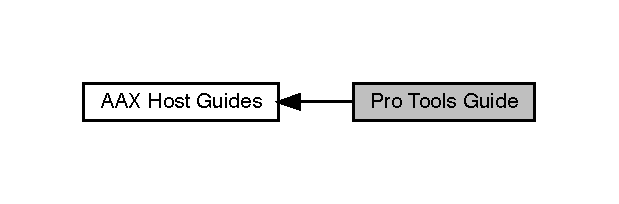
\includegraphics[width=297pt]{a00830}
\end{center}
\end{figure}
